\subsubsection{Geschichte}\label{devops_geschichte}

Das Wasserfallmodell stellt den klassischen Ansatz bei der Entwicklung von Software dar.
Dieser besteht aus den dargestellten aufeinanderfolgenden Stufen:

\begin{figure}[htb]
    \centering
    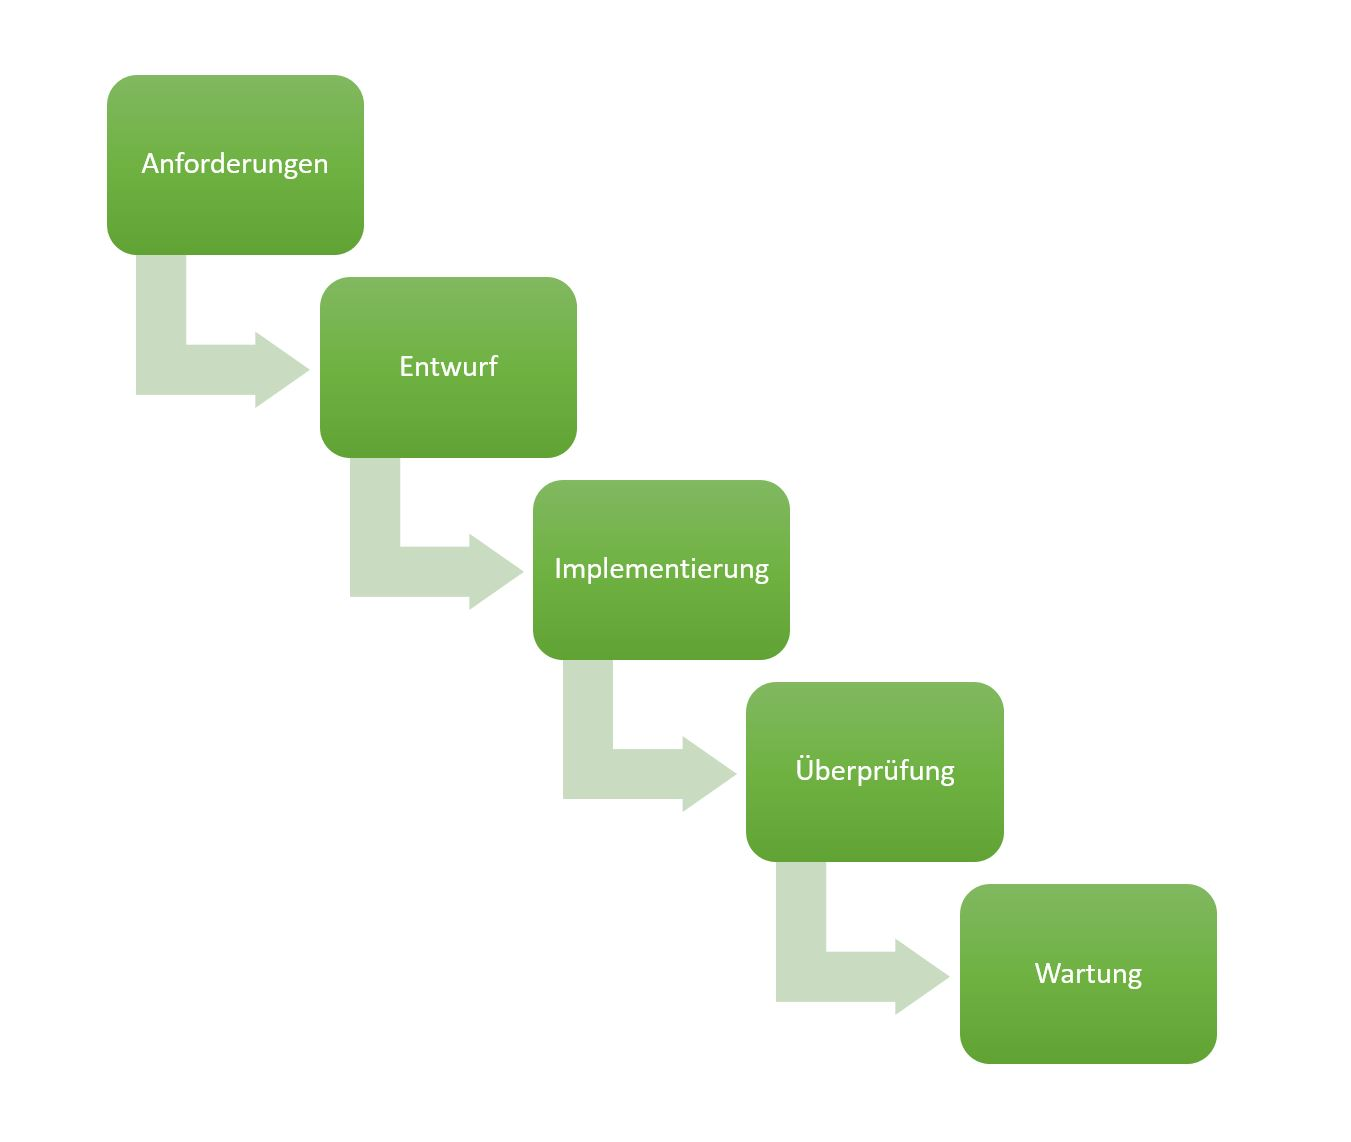
\includegraphics[width=0.8\textwidth]{images/wasserfall.jpg}
    \caption[Wasserfallmodell]{Wasserfallmodell}
    \label{fig:Wasserfallmodell}
\end{figure}

\begin{itemize}
    \item \textbf{Anforderungen:} Basierend auf einem Lasten- oder Pflichtenheft.
    \item \textbf{Entwurf:} Spezifikation und Dokumentation der Software.
    \item \textbf{Implementierung:} Entwicklung der Software auf Basis des Entwurfs.
    \item \textbf{Überprüfung:} Prüfung der Korrektheit mithilfe von Tests.
    \item \textbf{Wartung:} Pflege der Software mittels Updates bei Fehlern oder Sicherheitsproblemen.
\end{itemize}

Dieser Ansatz vernachlässigt, dass gerade in Unternehmen deren Hauptprodukt Software ist,
diese nie \textsl{fertig} ist und auch nach Fertigstellung der ersten Version weiterentwickelt werden muss.
\footnote{Kasteleiner/Schwartz, vgl.~\cite{Kasteleiner2019}~[S.211-214]}

Darüber hinaus hat das Modell die Einschränkung, dass die Phasen in der Realität nicht immer abgeschlossen werden können,
da die Anforderungen essenzieller Bestandteil für eine funktionierende Anwendung des Models sind.
Die Anforderungen müssen zuvor kommuniziert und festgelegt werden.
\footnote{Armenise, vgl.~\cite{Armenise2015}~[S.24]} \\

Im Buch: \textsl{The mythical man-month} von 1975, schreibt Fred Brooks: \footnote{Ozkaya, vgl.~\cite{Ozkaya2019}~[S.3]}

\begin{quotation}
    \textsl{Die meisten großen vergangenen Fortschritte in der Software Produktivität wurden durch das Entfernen von künstlichen Barrieren erreicht.}
\end{quotation}

Das \textsl{agile Manifest} wurde 2001 verfasst und basiert auf häufiger Auslieferung, leichtgewichtigen Prozessen und selbstmotivierten Teams statt wasserfallartiger Entwicklung.
\footnote{Kim et al., vgl.~\cite{Kim2018}~[S.4-5]}
Der Trend zur Beseitigung von Barrieren entstand als Unternehmen wie Netflix, Etsy und Spotify ihre Entwicklungspraktiken in Richtung DevOps und Lean implementierten.
\footnote{Lichtenberger, vgl.~\cite{Lichtenberger2017}~[S.245]}
Die sogenannten Lean Prinzipien haben sich in der Herstellung von physischen Gütern etabliert.
So wurden in den 80er Jahren weniger als 75\% der Bestellungen pünktlich ausgeliefert,
im Jahre 2005 ist dieser Wert sogar auf über 95\% gestiegen. \footnote{Kim et al., vgl.~\cite{Kim2018}~[S.3-5]}

Einer der Vorreiter in diesem Bereich war der Autohersteller Toyota.
Lean begann bei Toyota im Produktionsprozess (TPS).
Es handelt sich dabei um die Optimierung auf Material- und Informationsfluss statt Zerlegung in viele isolierte Arbeitsschritte.
\footnote{Samulat, vgl.~\cite{Samulat2017}~[S.206]}

Fokussiert wurde der Blick auf die Zeit (schneller Durchlauf des Materials) und die Qualität (beim ersten Mal richtig).
\footnote{Samulat, vgl.~\cite{Samulat2017}~[S.206]}

Als im Jahre 2009 die erste Konferenz zum Thema DevOps in Gent (Belgien) gehalten wurde,
war das Thema nicht ganz neu und wurde von Startups bereits vorgelebt. \footnote{Wiedemann, vgl.~\cite{Wiedemann2019}~[S.158]}
Die Konferenz bestand aus nur 60 Teilnehmer und galt als Start der DevOps-Bewegung,
die unter anderem von den Autoren des \textsl{DevOps Handbooks} wie z.B. Patrick Debois geprägt wurde.
\footnote{König/Kugel, vgl.~\cite{Konig2019}~[S.291]}

Ziel dieser Bewegung ist es, den Graben zwischen Entwicklung und Betrieb zum Wohle der Wertschöpfungskette zu schließen.
Das wird in der DevOps Bewegung auch als \textsl{Flow} bezeichnet. \footnote{Lichtenberger, vgl.~\cite{Lichtenberger2017}~[S.246]}
Dazu werden die sogenannten \textsl{Walls of Confusion}, also den Interessenskonflikten zwischen Entwicklung und Betrieb minimiert bzw. entfernt. \footnote{König/Kugel, vgl.~\cite{Konig2019}~[S.291]} \\

Moderne technische Projekte benötigen mehrere Perspektiven und Expertise. \footnote{Kim et al., vgl.~\cite{Kim2018}}
Die IT-Industrie stellt Prozesse immer noch infrage. \footnote{Samulat, vgl.~\cite{Samulat2017}~[S.206]},
Je weniger Zeremonien innerhalb eines Entwicklungsprozesses existieren, umso höher ist die Erfolgswahrscheinlichkeit. \footnote{Ozkaya, vgl.~\cite{Ozkaya2019}~[S.4]}
Diesen Umstand hat die DevOps-Bewegung erkannt, will dabei jedoch keine \textsl{One-Size-Fits-All}-Lösung sein. \footnote{König/Kugel, vgl.~\cite{Konig2019}~[S.291]}

%    [RESTE]
%    - experiencing increasing frustra- tion with delays and problems releas- ing software to production, while the operations team felt overloaded and constrained. `(Callanan, 53)`
%    - Gründe für DevOps: Digitalisierung, IT Abteilungen im Unternehmen gespalten `(Lichtenberger, 246)`
